\section{Introduction}
\label{sec:intro}

%{\newcommand\T{\rule{0pt}{4ex}}


Over the last few years, automatic construction of knowledge graphs (KGs) from web-scale text data has received considerable attention, resulting in the construction of several large KGs such as NELL \cite{mitchell2015never}, Google's Knowledge Vault \cite{dong2014knowledge}. These KGs consist of millions of entities and facts involving them. While measuring size of the KGs in terms of number of entities and facts is helpful, they don't readily capture the volume of knowledge needed in real-world applications. When such a KG is used in an application, one is often interested in known facts for a \emph{given} entity, and not necessarily the overall size of the KG. In particular, knowing the average number of facts per entity is quite informative. We shall refer to this as the \textit{knowledge density} of the KG. %Please note that a sparse KG will also have low knowledge density.

Low knowledge density (or high sparsity) in automatically constructed KGs has been recognized in recent research \cite{west2014knowledge}. For example, NELL KG has a knowledge density of 1.34. Such low knowledge density puts significant limitations on the utility of these KGs. Construction of such KGs tend to follow a batch paradigm: the knowledge extraction system makes a full pass over the text corpus extracting whatever knowledge it finds, and finally aggregating all extractions into a graph. Clearly, such \emph{best-effort} extraction paradigm has proved to be inadequate to address the low knowledge density issue mentioned above. We refer to such paradigm as best-effort since its attention is divided equally among all possible entities.

\begin{table}[t]
	\begin{center}
		{\small
		\begin{tabular}{|p{1.5cm}|C{2.2cm}|C{1.8cm}|}
		\hline
		& {\bf K}nown Target {\bf E}ntity & {\bf N}ew Target {\bf E}ntity \\
		\hline
		%\noalign{\vskip 2mm}
		{\bf K}nown {\bf R}elation & KR-KE & KR-NE \\
		\hline
		{\bf N}ew {\bf R}elation & NR-KE & NR-NE \\
		\hline
		\end{tabular}
		}		
\caption{\label{tbl:extraction_taxonomy}Any  new fact involving a source entity from a Knowledge Graph (i.e., facts of the form \textit{entity1-relation-entity2} where  \textit{entity1} is already in the KG) can be classified into one of the  four extraction classes shown above. Most KG population techniques tend to focus on extracting facts of the KR-KE class. \system{}, the entity-centric approach proposed in this paper, is able to extract facts of all four classes.}
	\end{center}
\end{table}
%}

\begin{figure*}[!htbp]
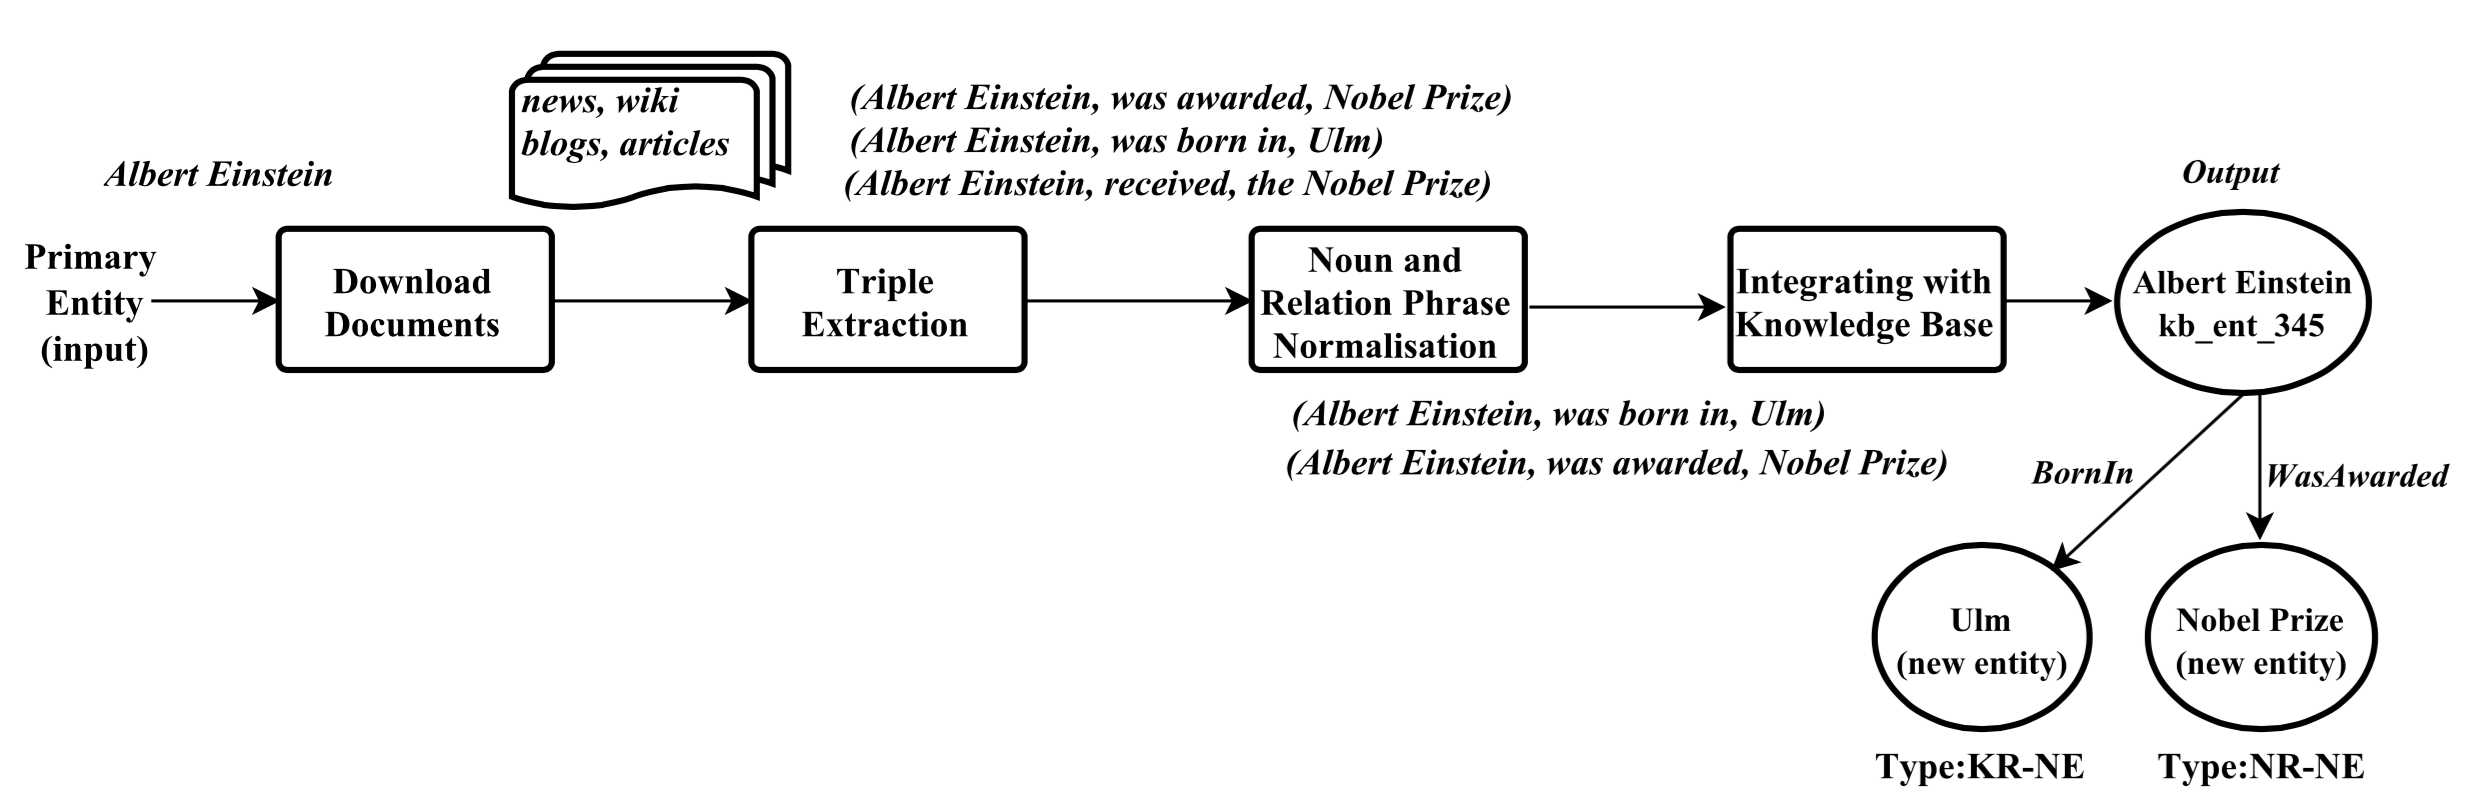
\includegraphics[scale= 0.36]{images/pipeline.png}
\caption{Dataflow and architecture and  of \system{}. See \refsec{sec:method} for details.}
\label{fig:pipeline}
\end{figure*}

Recently, a few \emph{entity-centric} methods have been proposed to increase knowledge density in KGs \cite{gardner2013improving,gardner2014incorporating}. In contrast to the best-effort approaches mentioned above, these entity-centric approaches aim at increasing knowledge density for a \emph{given} entity. A new fact involving the  given entity can belong to one of the four types  shown in \reftbl{tbl:extraction_taxonomy}. Unfortunately, these densifying techniques only aim at identifying instances of known relations among entities already present in the KG, i.e., they fall in the KR-KE type of \reftbl{tbl:extraction_taxonomy}.

In this paper we propose \systemfull{} (\system{}), an entity-centric knowledge densifying framework which, given an entity, is capable of extracting facts belonging to all the four types shown in \reftbl{tbl:extraction_taxonomy}. By using \system{}, we are able to increase NELL's knowledge density by a factor of 7.7\footnote{Measured with respect to the five categories experimented with in the paper. See \refsec{sec:expts} for details.}, while achieving 75.4\% accuracy. %While the framework itself is relatively simple and can be improved,
Our goal here is to draw attention to the effectiveness of entity-centric approaches with bigger scope (i.e., covering all four extraction classes  in \reftbl{tbl:extraction_taxonomy}) towards improving knowledge density, and that even relatively straightforward techniques can go a long way in alleviating low knowledge density in existing state-of-the-art KGs. \system{} code is available at: {\small {\tt https://github.com/malllabiisc/entity-centric- kb-pop}} %\textit{https://github.com/Manjunathhegde/entity-centric-kb-pop}

% They either focus on identifying instances of of known relations among known entities in the KG \cite{gardner2013improving,gardner2014incorporating}, or they require proprietary technologies not available in the public domain \cite{west2014knowledge}.

%While the knowledge density may be computed directly from the number of entities and facts in the KG, we feel it is an important metric which needs to be reported independently. Knowledge densities of a few KGs are shown in 

%A large number of knowledge base (KB) construction projects have recently emerged. Prominent examples include Freebase which powers the Google Knowledge Graph, 
%ConceptNet, YAGO and others. These KBs contain many millions of entities, organized in hundreds to hundred thousands of semantic classes, and hundred millions of relational facts between entities. 
%The approach towards building these knowledge bases is to collect all possible information from the corpus and represent them in the KB. Our approach in constructing entity specific 
%knowledge base is to search for the predefined entities and extract facts related to that. We store the extractions in the form of triples. For the primary entity, extractions will be of the form - (primary entity, relation, entity-2)
%or (entity-2, relation, primary entity)
%Finding the (relation, entity-2) pairs for the given primary entity and classifying them as new or existing information is the aim of this paper. 
%The set of operations are carried out on the subject verb object triples to find the relations and entity-2.
%NELL has the facts related to lot of entities, hence we use it to classify extractions as new or existing fact.
%With the (relation, entity-2) pair gives 5 different combination.\\
%Case 1: both the relation and entity-2 exists in the knowledge base and they are connected. So it is a known fact.
%Case 2: both the relation and entity-2 exists in the knowledge base but they are not connected. So it is a new fact.
%Case 3: relation is present in the KB but entity-2 is new. So system has identified a new entity.
%Case 4: entity-2 is present in the KB but relation is new. So system has identified a new relation.
%Case 5: both entity-2 and relation are new.
%The other sections describe the related work on this topic, methodology in clustering the data and mapping to existing knowledge base.
